%%%%%%%%%%%%%%%%%%%%%%%%%%%%%%%%%%%%%%%%%%%%%%%%%%%%%%%%%%%%%%%%%%%%%%%%%%%%%%%
%
% Filename: template.tex
% Author:   David Oniani
% Modified: January 24, 2021
%  _         _____   __  __
% | |    __ |_   _|__\ \/ /
% | |   / _` || |/ _ \\  /
% | |__| (_| || |  __//  \
% |_____\__,_||_|\___/_/\_\
%
%%%%%%%%%%%%%%%%%%%%%%%%%%%%%%%%%%%%%%%%%%%%%%%%%%%%%%%%%%%%%%%%%%%%%%%%%%%%%%%

%%%%%%%%%%%%%%%%%%%%%%%%%%%%%%%%%%%%%%%%%%%%%%%%%%%%%%%%%%%%%%%%%%%%%%%%%%%%%%%
% Document Definition
%%%%%%%%%%%%%%%%%%%%%%%%%%%%%%%%%%%%%%%%%%%%%%%%%%%%%%%%%%%%%%%%%%%%%%%%%%%%%%%

\documentclass[11pt]{article}

%%%%%%%%%%%%%%%%%%%%%%%%%%%%%%%%%%%%%%%%%%%%%%%%%%%%%%%%%%%%%%%%%%%%%%%%%%%%%%%
% Packages and Related Settings
%%%%%%%%%%%%%%%%%%%%%%%%%%%%%%%%%%%%%%%%%%%%%%%%%%%%%%%%%%%%%%%%%%%%%%%%%%%%%%%

% Global, document-wide settings
\usepackage[margin=1in]{geometry}
\usepackage[utf8]{inputenc}
\usepackage[english]{babel}

% Other packages
\usepackage{booktabs}
\usepackage{hyperref}
\usepackage{mathtools}
\usepackage{amsthm}
\usepackage{amssymb}
\usepackage{tikz}
\usepackage[cache=false]{minted}

%%%%%%%%%%%%%%%%%%%%%%%%%%%%%%%%%%%%%%%%%%%%%%%%%%%%%%%%%%%%%%%%%%%%%%%%%%%%%%%
% Command Definitions and Redefinitions
%%%%%%%%%%%%%%%%%%%%%%%%%%%%%%%%%%%%%%%%%%%%%%%%%%%%%%%%%%%%%%%%%%%%%%%%%%%%%%%

% Nice-looking underline
\newcommand\und[1]{\underline{\smash{#1}}}

% Line spacing is 1.5
\renewcommand{\baselinestretch}{1.5}

% Absolute value
\DeclarePairedDelimiter\abs{\lvert}{\rvert}%

% Absolute value big
\DeclarePairedDelimiter\absb{\Big\lvert}{\Big\rvert}%

% Ceiling
\DeclarePairedDelimiter{\ceil}{\lceil}{\rceil}

% Ceiling big
\DeclarePairedDelimiter{\ceilb}{\Big\lceil}{\Big\rceil}

% Floor
\DeclarePairedDelimiter\floor{\lfloor}{\rfloor}

% % Naturals, Reals, Integers, and Rationals, 
\newcommand{\nats}{\mathbb{N}}
\newcommand{\reals}{\mathbb{R}}
\newcommand{\preals}{\mathbb{R^+}}
\newcommand{\nreals}{\mathbb{R^-}}
\newcommand{\ints}{\mathbb{Z}}
\newcommand{\pints}{\mathbb{Z^+}}
\newcommand{\nints}{\mathbb{Z^-}}
\newcommand{\rats}{\mathbb{Q}}
\newcommand{\prats}{\mathbb{Q^+}}
\newcommand{\nrats}{\mathbb{Q^-}}
\newcommand{\irrats}{\mathbb{I}}
\newcommand{\pirrats}{\mathbb{I^+}}
\newcommand{\nirrats}{\mathbb{I^-}}

%%%%%%%%%%%%%%%%%%%%%%%%%%%%%%%%%%%%%%%%%%%%%%%%%%%%%%%%%%%%%%%%%%%%%%%%%%%%%%%
% Miscellaneous
%%%%%%%%%%%%%%%%%%%%%%%%%%%%%%%%%%%%%%%%%%%%%%%%%%%%%%%%%%%%%%%%%%%%%%%%%%%%%%%

% Setting stuff
\setlength{\parindent}{0pt}  % Remove indentations from paragraphs

% PDF information and nice-looking urls
\hypersetup{%
  pdfauthor={David Oniani},
  pdftitle={Real Analysis},
  pdfsubject={Mathematics, Real Analysis, Real Numbers},
  pdfkeywords={Mathematics, Real Analysis, Real Numbers},
  pdflang={English},
  colorlinks=true,
  linkcolor={black!50!blue},
  citecolor={black!50!blue},
  urlcolor={black!50!blue}
}

%%%%%%%%%%%%%%%%%%%%%%%%%%%%%%%%%%%%%%%%%%%%%%%%%%%%%%%%%%%%%%%%%%%%%%%%%%%%%%%
% Author(s), Title, and Date
%%%%%%%%%%%%%%%%%%%%%%%%%%%%%%%%%%%%%%%%%%%%%%%%%%%%%%%%%%%%%%%%%%%%%%%%%%%%%%%

% Author(s)
\author{David Oniani\\
        Luther College\\
        \href{mailto:oniada01@luther.edu}{oniada01@luther.edu}}

% Title
\title{\rule{\paperwidth - 150pt}{1pt}\textbf{\\\textit{Real Analysis
Exams}\\}\rule {\paperwidth - 150pt}{1pt}\\\textbf{Exam
\textnumero4}\\{\normalsize Instructor: Dr. Eric Westlund}}

% Date
\date{\today}

%%%%%%%%%%%%%%%%%%%%%%%%%%%%%%%%%%%%%%%%%%%%%%%%%%%%%%%%%%%%%%%%%%%%%%%%%%%%%%%
% Beginning of the Document
%%%%%%%%%%%%%%%%%%%%%%%%%%%%%%%%%%%%%%%%%%%%%%%%%%%%%%%%%%%%%%%%%%%%%%%%%%%%%%%

\begin{document}
\maketitle

%%%%%%%%%%%%%%%%%%%%%%%%%%%%%%%%%%%%%%%%%%%%%%%%%%%%%%%%%%%%%%%%%%%%%%%%%%%%%%%

\begin{itemize}
    \item[1.]
        \begin{itemize}
            \item[(a)]
                Notice that we have:
                \begin{align*}
                    \lim \sup a_n &= \lim_{n \to \infty} \Big(4 +
                                        \frac{1}{n}\Big) \cos
                                            \Big(\frac{n\pi}{4}\Big)
                                                = 4 \times 1 = 4
                \end{align*}
                Similarly, $\lim \inf a_n = 4 \times (-1) = -4$. Hence, $\lim
                \sup a_n = 4$ and $\lim \inf a_n = -4$.

            \item[(b)]
                Notice that the subsequence $a_k = \Big(4 +
                \dfrac{1}{8k}\Big)\cos (2\pi k)$ ($n = 8k$ with $k \in \nats$)
                converges to $0$ since $\cos (2\pi k) = 0$ and thus, every $a_k
                = \Big(4 + \dfrac{1}{8k}\Big) \times 0 = 0$.

            \item[(c)]
                This set will be $A = (-4, 4)$.
        \end{itemize}

    \clearpage

    \item[2.]
        Let $\epsilon > 0$ be given, $x_0$ be fixed, and let $\delta = \min
        \Big(1, \dfrac{\epsilon}{5(1 + 2\abs{x_0})}\Big)$. Then for $\abs{x -
        x_0} < \delta$ we have:
        \begin{align*}
            \abs{f(x) - f(x_0)} &= \abs{5x^2 + 3 - 5x_0^2 - 3}\\
                                &= \abs{5 (x^2 - x_0^2)}\\
                                &= 5 \abs{x - x_0} \abs{x - x_0 + 2x_0}\\
                                &< 5 \delta (\abs{x - x_0} + \abs{2x_0})\\
                                &< 5 \delta (\delta + 2\abs{x_0})\\
                                &\leq 5 \frac{\epsilon}{5(1 + 2\abs{x_0})} (\delta + 2\abs{x_0})\\
                                &\leq \frac{\epsilon}{1 + 2\abs{x_0}} (1 + 2\abs{x_0})\\
                                &= \epsilon
                                \tag{Thus, $\abs{f(x) - f(x_0)} < \epsilon$}
        \end{align*}
        Hence, $f(x) = 5x^2 + 3$ is continuous at each point $x_0 \in
        \reals$.\\
        $\qed$

    \item[3.]
        \begin{itemize}
            \item[(a)]
                Counterexample: let us define
                \begin{equation*}
                    f_n : [0, 1] \to \reals : x \mapsto
                    \begin{cases}
                        n &\text{ if } 0 < x < \dfrac{1}{n}\\
                        0 &\text{ if $x = 0$ or $\dfrac{1}{n} \leq x \leq 1$}
                    \end{cases}
                \end{equation*}
                Then notice that $\int_0^1 f_n = 1$ and the pointwise limit of
                $f_n$ is $f(x) = 0$ ($x \in [0, 1]$) for which we have
                $\int_0^1 f = 0$. Hence, we have $\int_0^1 f_n \to 1 \neq
                \int_0^1 f = 0$. Finally, we get that every $f_n$ is
                Riemann-integrable, but $f$ is not.

            \item[(b)]
                As $f_n \to f$ uniformly, pick $n_1$ s.t. the following holds:
                \begin{equation*}
                  \abs{f_{n_1}(x) - f(x)} < \frac{\epsilon}{3\cdot(b-a)}
                \end{equation*}
                Now, since every $f_n$ is integrable, take $n_2$ such that
                \begin{equation*}
                  \abs{U(f_{n_1}, P_{n_2}) - L(f_{n_1}, P_{n_2})} <
                        \frac{\epsilon}{3}.
                \end{equation*}
                Now, choose $n = \max(n_1, n_2)$,

                Notice that 
                \begin{align*}
                    \abs{
                        U(f, P_{n}) - U(f_n, P_{n})
                    } 
                    &\leq \sum_{x_k} \abs{f(x_k) - f_n(x_k)} \Delta x_k\\
                    &< \sum_{x_k} \frac{\epsilon}{3(b-a)} \Delta x_k\\
                    &= \frac{\epsilon}{3(b-a)} \sum_{x_k} \Delta x_k\\
                    &= \frac{\epsilon}{3(b-a)} (b-a)\\
                    &= \frac{\epsilon}{3}
                \end{align*}
                Now, notice that over $[x_k, x_{k+1}]$, $\abs{\sup f(x) - \sup
                f_n(x)} \leq \abs{f_{n}(x) - f(x)}$ (since every point of $f_n$
                is close to $f$).

                A similar results holds for
                \begin{equation*}
                  \abs{L(f, P_{n_2}) - L(f_n, P_{n_2})}  < \frac{\epsilon}{3}
                \end{equation*}

                Hence, we have:
                \begin{align*}
                  \abs{U(f, P_n) - L(f, P_n)} &\leq 
                  \absb{U(f, P_n) - U(f_n, P_n) + U(f_n, P_n) - L(f_n, P_n) -
                      \Big(L(f, P_n) - L(f_n, P_n)\Big)}\\
                  &\leq \abs{ U(f, P_n) - U(f_n, P_n) } + \abs{ U(f_n, P_n) -
                      L(f_n, P_n) } + \abs{ L(f, P_n) - L(f_n, P_n) }\\
                  &< \frac{\epsilon}{3} + \frac{\epsilon}{3} +
                     \frac{\epsilon}{3} = \epsilon
                \end{align*}
                Finally, we got that if $f_n \to f$ uniformly on $[a, b]$, then
                $f$ is integrable on $[a, b]$.\\
                $\qed$

            \item[(c)]
                We have already shown in $(b)$ part of the exercise that $f$ is
                integrable on $[a, b]$. We now need to show that the following
                holds:
                \begin{equation*}
                  \lim_{n\to \infty} \int_a^b f_n = \int_a^b f
                \end{equation*}
                It follows by the uniform convergence of $f_n$ that
                \begin{align}
                    \abs{f_n - f} &< \epsilon &\implies& f - \epsilon < f_n <
                    f + \epsilon\\
                    \int_a^b \Big(f - \epsilon\Big) &< \int_a^b f_n < \int_a^b
                    \Big(f + \epsilon\Big) &\implies& \absb{\int_a^b f_n -
                    \int_a^b f} < \epsilon(b - a)
                \end{align}
                Hence, we can make the difference $\abs{\int_a^b f_n - \int_a^b
                f}$ arbitrarily small and we get $\lim_{n\to \infty} \int_a^b
                f_n = \int_a^b f$.\\
                $\qed$
        \end{itemize}

    \item[4.]
        Yes, $G$ is differentiable at $1$. In order to show this, we must show
        that the following limit exists:
        \begin{equation*}
            \lim_{x \to 1} \frac{G(x) - G(1)}{x - 1}
        \end{equation*}
        Notice that the antiderivative $A$ of function $g$ can be calcuated as:
        \begin{equation*}
            A =
            \begin{cases}
                x  &\text{ if } x \neq 1\\
                2x &\text{ if } x = 1
            \end{cases}
        \end{equation*}
        We have:
        \begin{align*}
            G(1) = \int_0^1 g = A^\prime(1) - A^\prime(0) = 2 - 1 = 1
        \end{align*}
        Plugging in the values into the limit formula above, we get:
        \begin{equation*}
            \lim_{x \to 1} \frac{\int_0^x g - 1}{x - 1}
        \end{equation*}
        Now, clearly $\lim_{x \to 1^-} \frac{1 - 1}{x - 1} = 0$ and $\lim_{x
        \to 1^+} \frac{1 - 1}{x - 1} = 0$. Hence, $\lim_{x \to 1}
        \frac{\int_0^x g - 1}{x - 1} = 0$ and always exists. Finally, we got
        that $G$ is differentiable at $1$.\\
        $\qed$

    \item[5.]
        No, $H$ is not differentiable at $1$. In order to show this, we must
        show that the following limit does not exist:
        \begin{equation*}
            \lim_{x \to 1} \frac{H(x) - H(1)}{x - 1}
        \end{equation*}
        Notice that the antiderivative $A$ of function $h$ can be calcuated as:
        \begin{equation*}
            A =
            \begin{cases}
                x  &\text{ if } x < 1\\
                2x &\text{ if } x \geq 1
            \end{cases}
        \end{equation*}
        We have:
        \begin{align*}
            G(1) = \int_0^1 g = A^\prime(1) - A^\prime(0) = 2 - 1 = 1
        \end{align*}
        Plugging in the values into the limit formula above, we get:
        \begin{equation*}
            \lim_{x \to 1} \frac{\int_0^x h - 1}{x - 1}
        \end{equation*}
        Now, clearly $\lim_{x \to 1^-} \frac{1 - 1}{x - 1} = 0$ and $\lim_{x
        \to 1^+} \frac{1 - 2}{x - 1} \neq 0$. Hence, $\lim_{x \to 1^-} \neq
        \lim_{x \to 1^+}$ and the two-sided limits are not the same which
        implies that the limit does not exist. Finally, we got that $H$ is not
        differentiable at $1$.\\
        $\qed$

    \item[6.]
        Let $A(t)$ be the antiderivative of $t^2\sin (t^2)$. We have:
        \begin{align*}
            \frac{d}{dx} \int_0^{x^2} t^2\sin (t^2) dt
                &= \frac{d}{dx} A(x^2) - A(0)\\
                &= 2x A^\prime(x^2)\\
                &= 2x \times (x^2)^2 \sin ((x^2)^2\\
                &= 2x^5 \sin (x^4)
        \end{align*}

    \item[7.]
        Since $f$ is continuous on $[a, b]$, it follows that $f$ achieves both
        the absolute maximum $M$ and the absolute minimum $m$ in $[a, b]$.
        Suppose, without a loss of generality, that these points are $c_1$ and
        $c_2$ with $c_1 < c_2$. We then have:
        \begin{align}
            m (b - a) \leq \int_a^b f \leq M (b - a)\\
            m \leq \frac{1}{b - a} \int_a^b f \leq M
        \end{align}
        Now, it follows by \textbf{Intermediate Value Theorem} that $\exists c
        \in (c_1, c_2) \subset [a, b]$ s.t. $f(c) = \frac{1}{b - a} \int_a^b
        f$.\\
        $\qed$

    \item[8.]
        Suppose, for the sake of contradiction, that $f$ has Generalized
        Riemann integrals $Q_1$ and $Q_2$ with $Q_1 \neq Q_2$ and let $\epsilon
        > 0$ be given. Then,.it follows that $\exists \delta_1(x)$ s.t.
        $\forall \delta_1(x)$-fine tagged partitions, $\abs{R(f, P) - Q_1} <
        \frac{\epsilon}{2}$. Similarly, $\exists \delta_2(x)$ s.t. $\forall
        \delta_2(x)$-fine tagged partitions, $\abs{R(f, P) - Q_2} <
        \frac{\epsilon}{2}$. Now, let $\delta(x) = \min (\delta_1(x),
        \delta_2(x))$. It follows by \textbf{Theorem 8.1.5} that there exists a
        tagged partition $(P, \{c_k\})$ s.t. it is both $\delta_1(x)$-fine and
        $\delta_2(x)$-fine. We have:
        \begin{equation*}
            \abs{Q_1 - Q_2} \leq \abs{Q_1 - R(f, P)} + \abs{R(f, P) - Q_2}
                            < \frac{\epsilon}{2} + \frac{\epsilon}{2}
                            = \epsilon
        \end{equation*}
        Hence, we got that $Q_1 = Q_2$ and we face a contradiction since we
        have assumed that $Q_1 \neq Q_2$. Finally, we conclude that if $f$ has
        a generalized Riemann integral on $[a, b]$, then the value of the
        integral $\int_a^b f$ is unique.\\
        $\qed$

    \clearpage

    \item[9.]
        \begin{itemize}
            \item[(a)]
                Below find the plots.

                \begin{figure}[H]
                    \centering
                    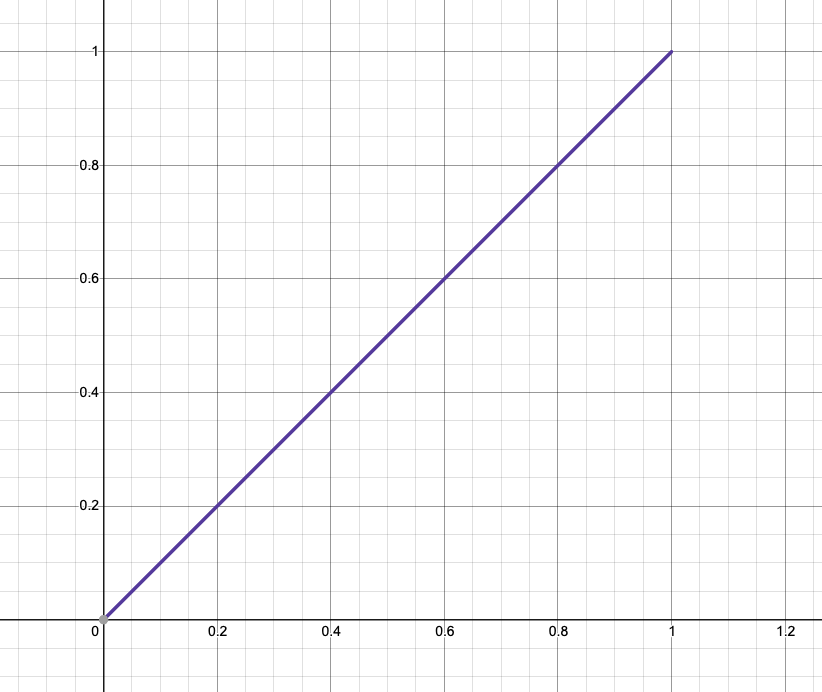
\includegraphics[width=0.5\linewidth]{f_0_plot.png}
                    \caption{Plot of $f_0$}
                \end{figure}

                \begin{figure}[H]
                    \centering
                    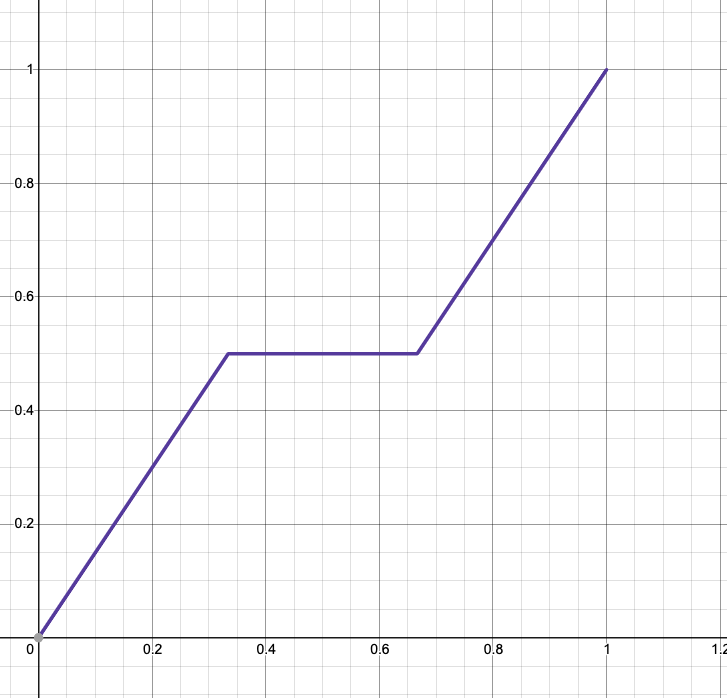
\includegraphics[width=0.5\linewidth]{f_1_plot.png}
                    \caption{Plot of $f_1$}
                \end{figure}

                \begin{figure}[H]
                    \centering
                    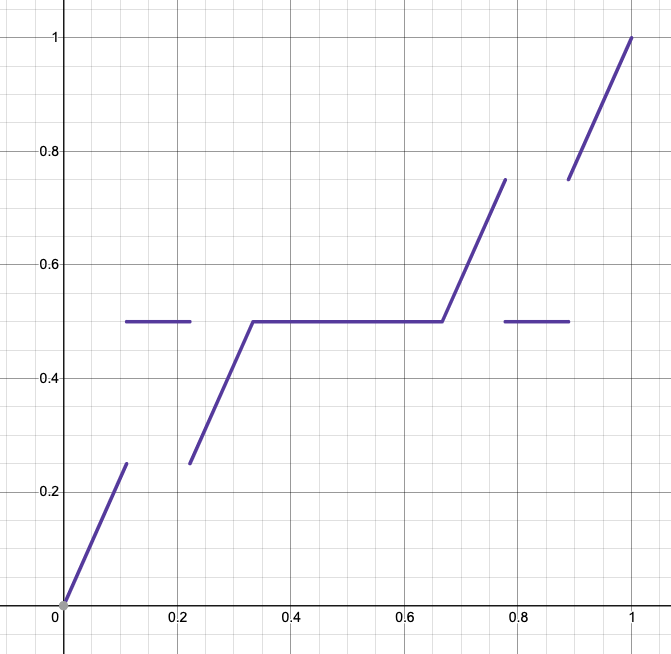
\includegraphics[width=0.5\linewidth]{f_2_plot.png}
                    \caption{Plot of $f_2$}
                \end{figure}

            \item[(b)]
                \begin{equation*}
                    f_3(x) =
                    \begin{cases}
                        \dfrac{f_2(3x)}{2}
                            &\text{ if } 0 \leq x \leq \dfrac{1}{3}\\
                        \dfrac{1}{2}
                            &\text{ if } \dfrac{1}{3} < x < \dfrac{2}{3}\\
                        \dfrac{(f_2(3x - 3) + 2)}{2}
                            &\text{ if } \dfrac{2}{3} \leq x \leq 1
                    \end{cases}
                \end{equation*}

                Below find the graph of $f_3$:
                \begin{figure}[H]
                    \centering
                    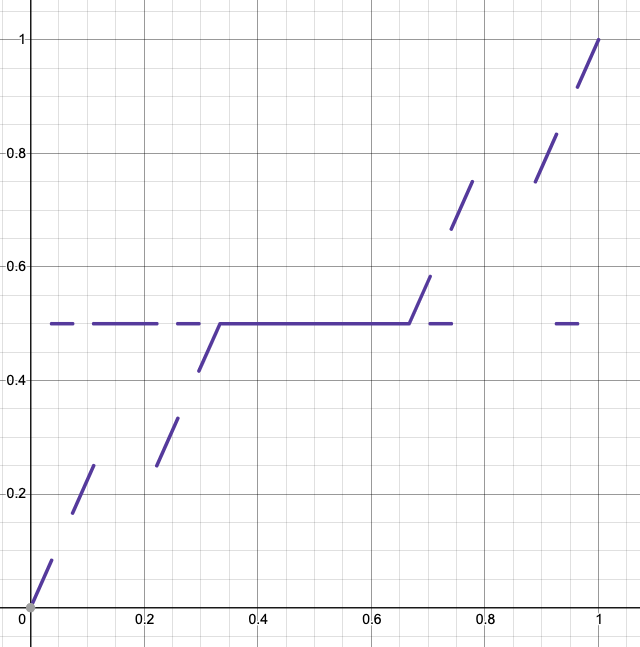
\includegraphics[width=0.45\linewidth]{f_3_plot.png}
                    \caption{Plot of $f_3$}
                \end{figure}

            \item[(c)]
                It is similar to the cantor set in a way that the function
                iteratively turns the open middle third of its values to
                $\dfrac{1}{2}$.
                \\
                \\
                The difference is that in Cantor's set, the open middle third
                was completely removed, but in this case it is just transformed
                into $\dfrac{1}{2}$.

            \item[(d)]
                Notice that at each step, the function just turns some
                portion(s) of the closed interval $[0, 1]$ into $\dfrac{1}{2}$.
                Hence, there are no discontinuities and the function has to be
                continuous.\\
                $\qed$

            \item[(e)]
                The function is not differentiable at non-endpoints of $[0,
                1]$. Hence, we have:
                \begin{equation*}
                    f^\prime(x) = 
                    \begin{cases}
                        0    &\text{ if } x \in \{0, 1\}\\
                        none &\text{ otherwise}
                    \end{cases}
                \end{equation*}
                Now, let us show that the function is not differentiable at
                non-endpoints. Suppose, for the sake of contradiction,
                $(x_n) \to x$ and $(y_n) \to x$ s.t. $\forall n, x_n < y_n$
                and asume that the derivative exists. We have:
                \begin{equation*}
                    \frac{f(y_n) - f(x_n)}{y_n - x_n} \to f^\prime(x)
                \end{equation*}
                Now, we can see that $y_n - x_n = \dfrac{1}{3^n}$, but $f(y_n)
                - f(x_n) = \dfrac{1}{2^n}$, hence $f^\prime(x) \to \infty$ and
                we face the contradiction. Thus, the derivative cannot exist.\\
                $\qed$

            \item[(f)]
                As mentioned in $(d)$, as $n$ approaches infinity, all of the
                interval $[0, 1]$ will be $\frac{1}{2}$. Notice that $\forall n
                \in \nats$ (including $n \to \infty$), $f(0) = 0$ and $f(1) =
                1$. To see this, one could think about the graph construction
                or about the fact that in the end, for $x = 0$, the function
                will have a multiplication by $0$ (yields $0$), similar
                reasoning could be applied for obtaining $f(1) = 1$.
                Hence, we have:
                \begin{equation*}
                    \int_0^1 f = f(1) - f(0) = 1 - 0 = 1
                \end{equation*}
                Even easier way to see that $\int_0^1 f = 1$ is to notice that
                the function itself does not remove any points from the
                interval $[0, 1]$, it just maps to $\frac{1}{2}$ and hence, the
                total number of points always stays the same.
        \end{itemize}
\end{itemize}

%%%%%%%%%%%%%%%%%%%%%%%%%%%%%%%%%%%%%%%%%%%%%%%%%%%%%%%%%%%%%%%%%%%%%%%%%%%%%%%
% The End of the Document
%%%%%%%%%%%%%%%%%%%%%%%%%%%%%%%%%%%%%%%%%%%%%%%%%%%%%%%%%%%%%%%%%%%%%%%%%%%%%%%

\end{document}
